\documentclass{article}
\author{Bruno Berastain}
\usepackage{amsmath, amssymb, amsthm, tikz}

\begin{document}
\title{Using K-Nearest Neighbors and Linear Regression to Predict Housing Prices}
\maketitle

\section{The Problem}
You're planning to move and it's time to sell your house. You want to set the highest price that will sell quickly. Price it too high, it will take a long time to sell. Price it too low, and you'll get less than the house is worth. How can you find the perfect price?

\section{Compare To Similar Houses}
% sub-section header: K-Nearest Neighbors
What if you looked at recently sold houses similar to yours? That would give you an idea of the price to list your house. Say you had information about 10 recently sold houses, including the prices at which they sold. You could find the house most similar to yours, and assume that your house would sell at the same price. How do you decide which house is most similar to yours? You could take a feature of the houses, like number of rooms, and organize them all on a number line from least to most rooms. Then you could put your house on the number line, and choose the same selling price as the house closest to yours. Assume the distribution of houses with different number of bedrooms was\\

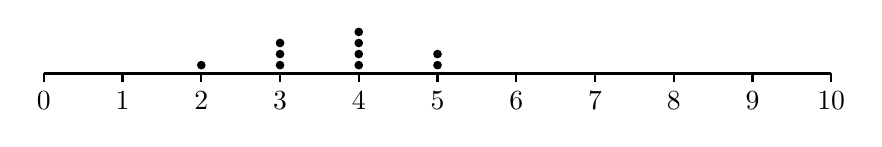
\begin{tikzpicture}[thick]
  \draw(0,0)--(10,0);
  \foreach \x in {0,1,...,10}
    \draw(\x,0pt)--(\x,-3pt) node[below] {\x};
  \foreach \x in {2,3,4,5}
  	\draw [fill] (\x,3pt) circle [radius=0.04];
  \foreach \x in {3,4,5}
  	\draw [fill] (\x,7pt) circle [radius=0.04];
  \foreach \x in {3,4}
  	\draw [fill] (\x,11pt) circle [radius=0.04];
  \draw [fill] (4,15pt) circle [radius=0.04];
\end{tikzpicture}\\

If your house has 4 rooms, you could pick the selling price of one of the other houses with 4 rooms. A better method might be to take the average selling price of all the houses with 4 rooms. Obviously number of bedrooms isn't enough to determine which house is most similar. Maybe your house has a large backyard and you're concerned the houses you're comparing it to don't reflect that, so you decide to look at square footage as well. Once again, you could plot all 10 houses on a graph, this time with number of bedrooms on the x-axis and square footage on the y-axis. Once again, you could plot your own house on there and find which house is the closest.

% graph of bedrooms
\begin{tikzpicture}[thick]
  \draw(0,6)--(0,0)--(6,0);
  \foreach \x in {1,...,6}
    \draw(\x,0pt)--(\x,-3pt) node[below] {\x};
  \foreach \x/\xtext in {1/500,2/600,3/700,4/800,5/900,6/1000}
    \draw(0,\x)--(-3pt,\x) node[left] {\xtext};
  \draw(3,-0.5) node[below] {Bedrooms};
  \draw(-1,4) node[left,rotate=90] {Square Feet};
\end{tikzpicture}\\

To determine how close a house is to yours you can use the distane formula 
\begin{equation}
  \(\sqrt{(x_{1}-x_{2})^2 + (y_{1}-y_{2})^2}\)
\end{equation}

The smaller the distance, the more similar it is. Once you know which houses are most similar, you can average a few of their prices to determine the price you'll set for your house. The letter "k" refers to the number of houses whose selling price you decide to average. This is where the algorithm "K-Nearest Neighbors" gets its name. (This won't work exactly as desired because the number of bedrooms is negligable compared to the number of square feet. The latter numbers are so much larger that the distance will barely be affected by the number of bedrooms. To correct for this, you can regularize all the variables, but for now you can ignore regularization.)\\

If you only have 10 houses to compare, you could likely rank the most similar ones yourself. But if you have 10,000 houses for comparison, you'll want to take into account as many features as you can. For a third feature, the distance formula would expand to \(\sqrt{(x_{1}-x_{2})^2 + (y_{1}-y_{2})^2 + (z_{1} - z_{2})^2\) and you could visualize the distance in three dimensional space. You can't visualize higher dimensions, but the distance formula can expand indefinitely
\begin{equation}
\(\sqrt{(x_{1}-y_{1})^2 + (x_{2}-y_{2})^2 + \cdots + (x_{n}-y_{n})^2}\)
\end{equation}
where x and y represent your house and the house you're measuring the distance to respectively, each with n features. Regardless of the number of features, the process is the same: Calculate the distance from each house to yours, choose the k-nearest, and average their selling price.






% We'll need a way to turn categorical variables into quantitative ones that can be used in the distance formula. - What's the other term for "dummy variables"?

% The set of 100 houses with known selling price that we used to determine our price is called the training set.
% The price, the variable we are trying to predict, is the target variable.
% All the aspects of the house 


\end{document}